\documentclass{article}
\usepackage{multicol}

\begin{document}
\chapter{Results}

PLSI has been implemented and works for multiple Rocket Chip based designs.
This section presents the results for Rocket, BOOM, and Hwacha on Synopsys'
32nm Educational PDK produced via the Synopsys tools.  In addition to
presenting the results, there is a discussion of the validity of the results.

These results were all run using the latest version of Rocket Chip that
supported the various configurations when this thesis was being written.  The
excat versions of Rocket Chip differ between the various targets because all
the forks aren't up to date at all times, but they're all tagged as git
submodules in the thesis repository.  Newer versions of Rocket Chip have
removed support for the L2 cache, which is why the Hwacha configuration (which
is based on an older version of Rocket Chip) is the only configuration that has
an L2 cache attached.

\subsection{Rocket}

\begin{figure}
  \begin{verbatim}
{
  "clocks": [
    {
      "name": "clock",
      "period": "1250ps",
      "par derating": "250ps"
    }
  ],
  "scenarios": [
    {
      "corner": {
        "nmos": "typical",
        "pmos": "typical",
        "temperature": "25 C"
      },
      "supplies": {
        "VDD": "1.05 V",
        "GND": "0 V"
      }
    }
  ]
}
\end{verbatim}
  \caption{PLSI CAD Configuration for DefaultConfig}
  \label{res:rocket-config}
\end{figure}

\begin{figure}
\tiny
\begin{verbatim}
class RocketTilePlacer:
  def __init__(self, config):
    self.top = None
    self.l1dd = []
    self.l1dm = []
    self.l1id = []
    self.l1im = []

  def insert(self, macro):
    if macro.matches(config.rtl_top):
      self.top = TopMacro(macro.name, macro.width, macro.height)
    # Version Break
    elif macro.matches("coreplex/RocketTile/DCache/data"):
      self.l1dd.append(macro)
    elif macro.matches("coreplex/RocketTile/DCache/MetadataArray"):
      self.l1dm.append(macro)
    elif macro.matches("coreplex/RocketTile/icache/icache"):
      self.l1id.append(macro)
    elif macro.matches("coreplex/RocketTile/icache/icache/tag_array/tag_array"):
      self.l1im.append(macro)
    # Version Break
    elif macro.matches("coreplex/rocketTiles/dcache/data"):
      self.l1dd.append(macro)
    elif macro.matches("coreplex/rocketTiles/dcache/MetadataArray"):
      self.l1dm.append(macro)
    elif macro.matches("coreplex/rocketTiles/frontend/icache"):
      self.l1id.append(macro)
    elif macro.matches("coreplex/rocketTiles/frontend/icache/u"):
      self.l1id.append(macro)
    elif macro.matches("coreplex/rocketTiles/frontend/icache/tag_array/tag_array"):
      self.l1im.append(macro)
    else:
      print("%s cannot be matched" % macro.name)
      return False
    return True

  def list_constraints(self):
    l1dd = TopLeftPlacer   (self.top, self.top.tlf(), sorted(self.l1dd), True)
    l1dm = TopLeftPlacer   (self.top, l1dd.bl(),      sorted(self.l1dm), False)
    l1id = BottomLeftPlacer(self.top, self.top.blf(), sorted(self.l1id), True)
    l1im = BottomLeftPlacer(self.top, l1id.tl(),      sorted(self.l1im), False)
    return l1dd.place() + l1dm.place() + l1id.place() + l1im.place()
\end{verbatim}
  \caption{PLSI Floorplan for DefaultConfig}
  \label{res:rocket-fppy}
\end{figure}

\begin{figure}
  \begin{center}
    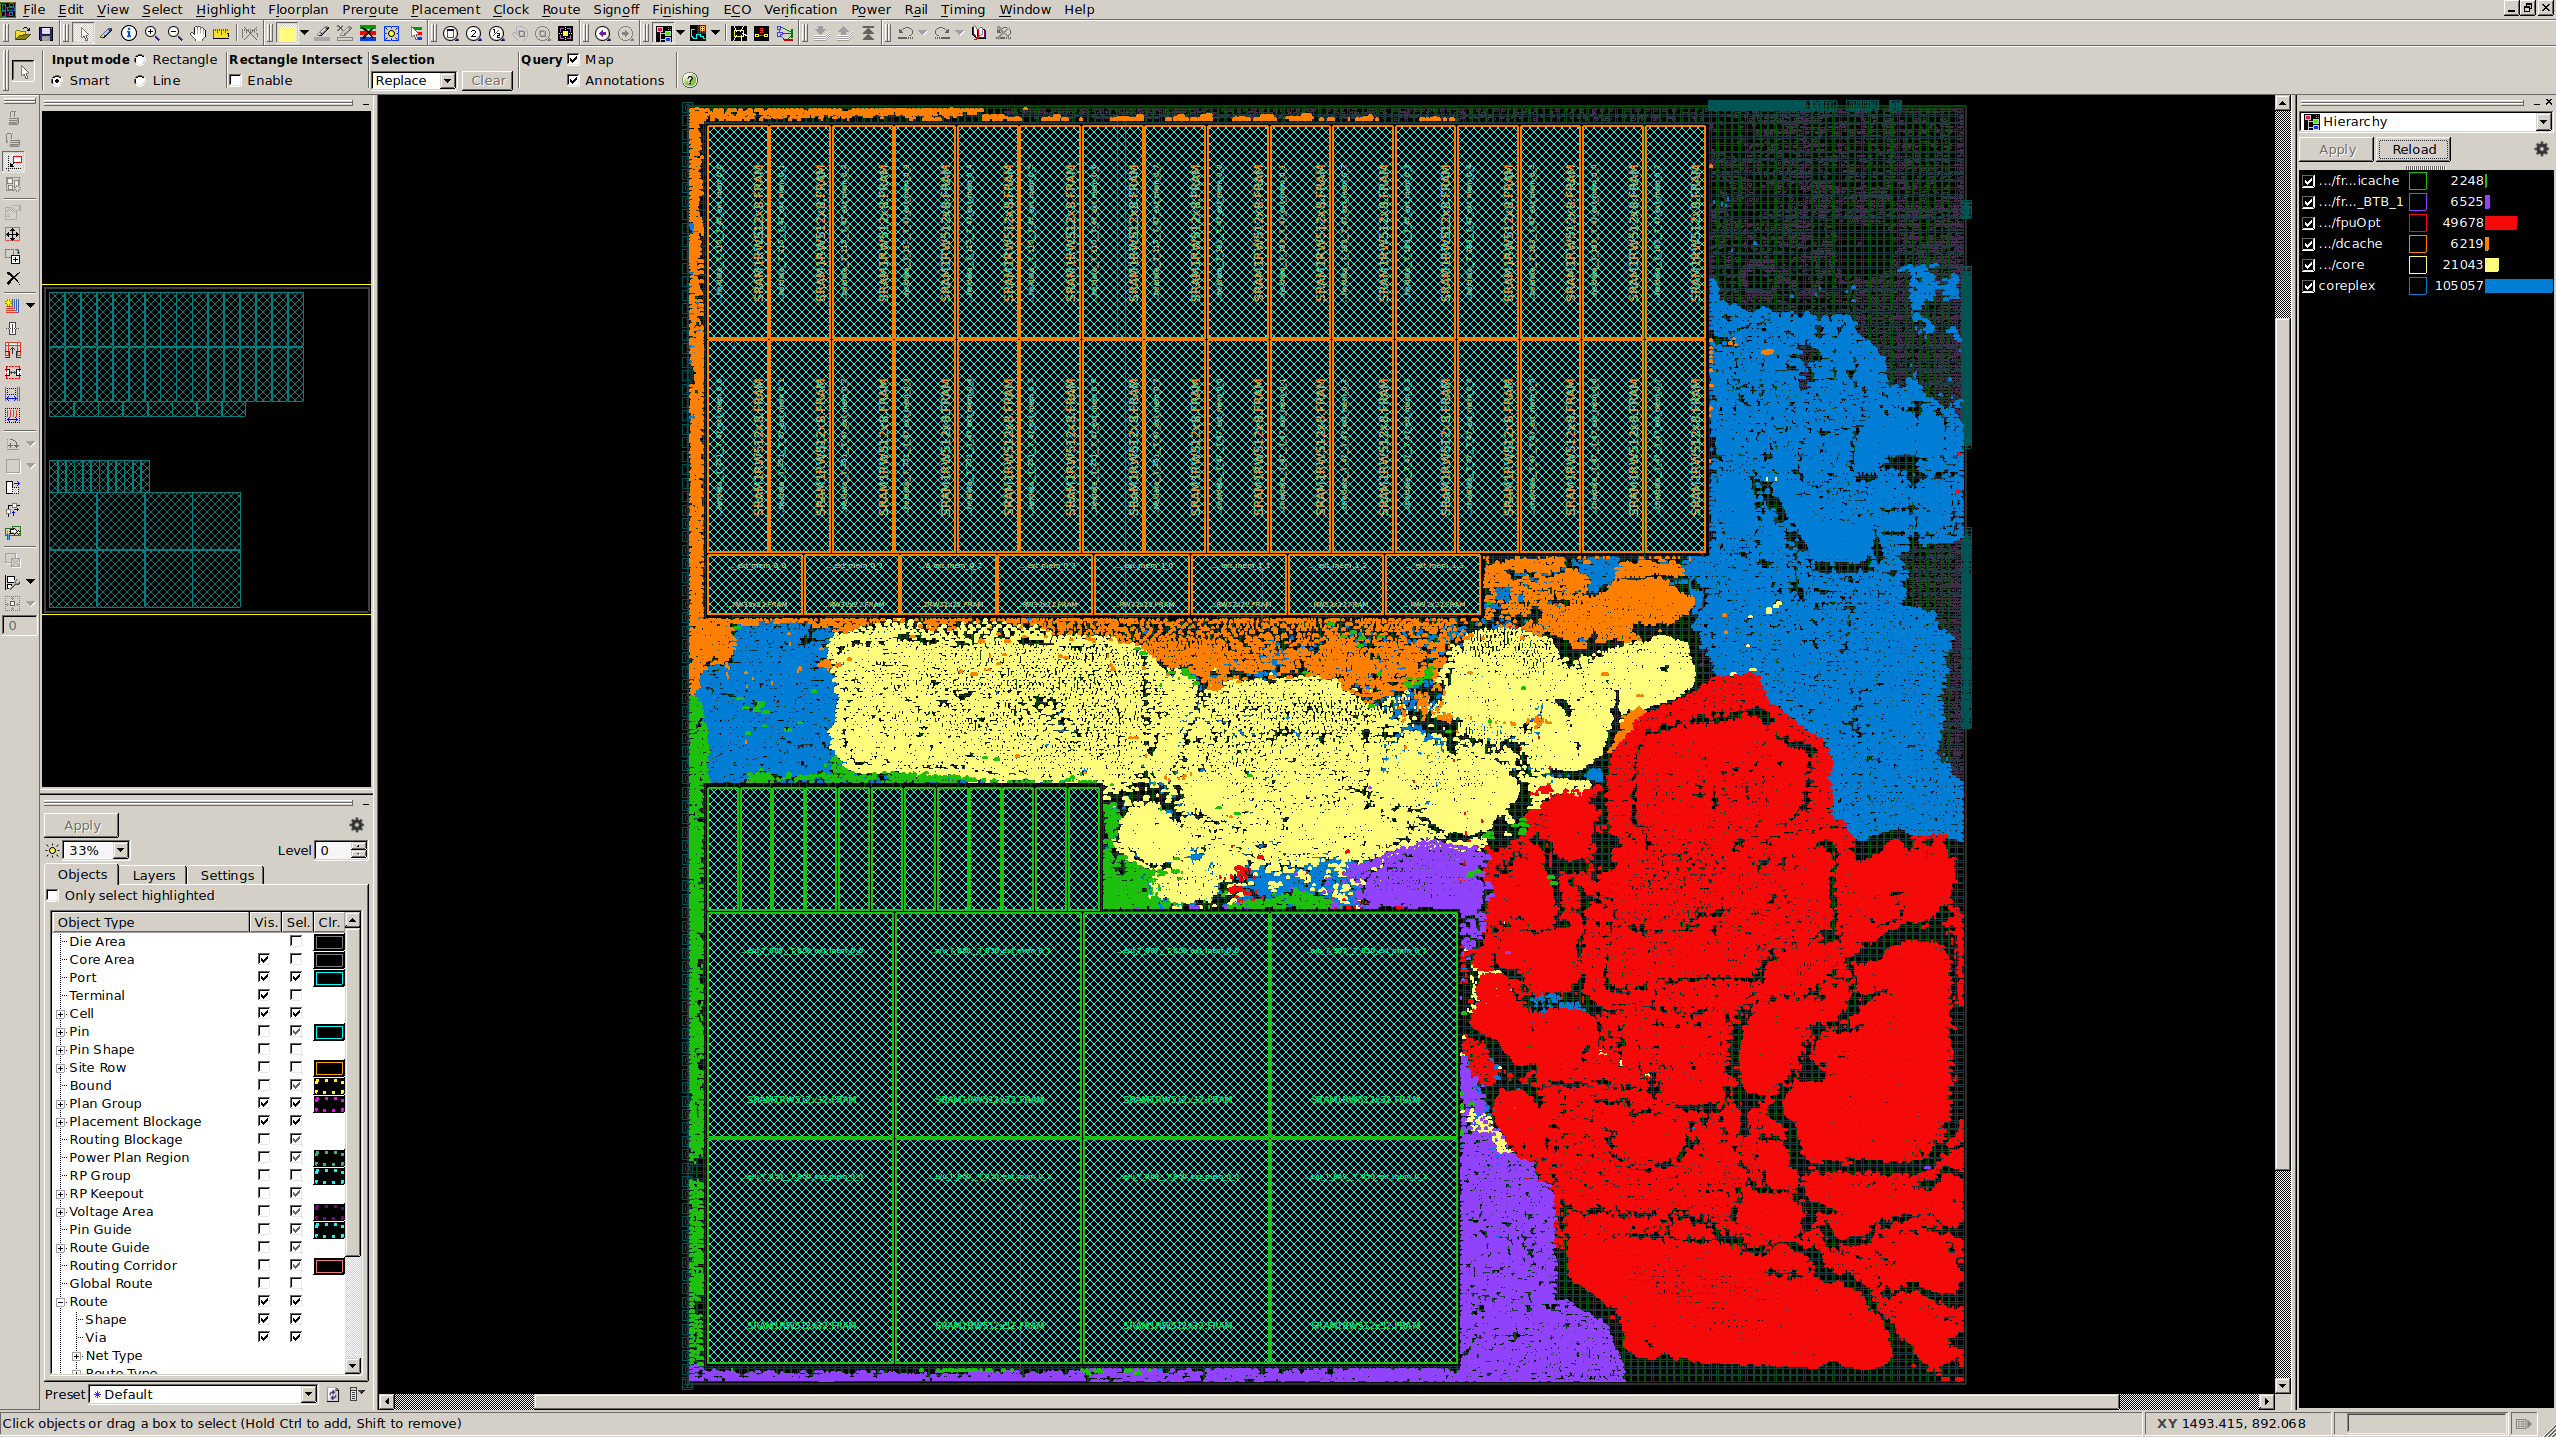
\includegraphics[width=0.95\linewidth]{figures/icc-rocket.png}
  \end{center}
  \caption{ICC Floorplan for DefaultConfig}
  \label{res:rocket-icc}
\end{figure}

\begin{figure}
\begin{multicols}{2}
\begin{verbatim}
  Timing Path Group 'clock'
  -----------------------------------
  Levels of Logic:              34.00
  Critical Path Length:          1.52
  Critical Path Slack:          -0.16
  Critical Path Clk Period:      1.35
  Total Negative Slack:        -18.73
  No. of Violating Paths:      988.00
  Worst Hold Violation:          0.00
  Total Hold Violation:          0.00
  No. of Hold Violations:        0.00
  -----------------------------------
\end{verbatim}

\begin{verbatim}
  Cell Count
  -----------------------------------
  Hierarchical Cell Count:        609
  Hierarchical Port Count:      18116
  Leaf Cell Count:             115987
  Buf/Inv Cell Count:           16638
  Buf Cell Count:                7235
  Inv Cell Count:                9403
  CT Buf/Inv Cell Count:          689
  Combinational Cell Count:     94266
  Sequential Cell Count:        21721
  Macro Count:                     60
  -----------------------------------
\end{verbatim}

\begin{verbatim}
  Area
  -----------------------------------
  Combinational Area:   258124.149879
  Noncombinational Area:
                        144030.016922
  Buf/Inv Area:          48915.350153
  Total Buffer Area:         31126.03
  Total Inverter Area:       17789.32
  Macro/Black Box Area:
                       1009378.968750
  Net Area:             381408.759989
  Net XLength        :     2435133.75
  Net YLength        :     2365051.00
  -----------------------------------
  Cell Area:           1411533.135552
  Design Area:         1792941.895541
  Net Length        :      4800185.00


  Design Rules
  -----------------------------------
  Total Number of Nets:        125786
  Nets With Violations:           316
  Max Trans Violations:            14
  Max Cap Violations:             308
\end{verbatim}
\end{multicols}
  \caption{ICC QoR Report for DefaultConfig}
  \label{res:rocket-qor}
\end{figure}

\subsection{BOOM}

\begin{figure}
  \begin{verbatim}
{
  "clocks": [
    {
      "name": "clock",
      "period": "1600ps",
      "par derating": "400ps"
    }
  ],
  "scenerios": [
    {
      "corner": {
        "nmos": "typical",
        "pmos": "typical",
        "temperature": "25 C"
      },
      "supplies": {
        "VDD": "1.05 V",
        "GND": "0 V"
      }
    }
  ]
}
\end{verbatim}
  \caption{PLSI CAD Configuration for SmallBOOMConfig}
  \label{res:boom-config}
\end{figure}

\begin{figure}
\tiny
\begin{verbatim}
class BoomTilePlacer(RocketTilePlacer):
  def __init__(self, config):
    self.top = None
    self.l1dd = []
    self.l1dm = []
    self.l1id = []
    self.l1im = []
    self.l1ht = []
    self.l1pt = []
    self.l1ei = []

  def insert(self, macro):
    if macro.matches(config.rtl_top):
      self.top = TopMacro(macro.name, macro.width, macro.height)
    # Version Break
    elif macro.matches("coreplex/BOOMTile/DCache/data"):
      self.l1dd.append(macro)
    elif macro.matches("coreplex/BOOMTile/DCache/MetadataArray"):
      self.l1dm.append(macro)
    elif macro.matches("coreplex/BOOMTile/HellaCache/MetadataArray"):
      self.l1dm.append(macro)
    elif macro.matches("coreplex/BOOMTile/HellaCache/meta"):
      self.l1dm.append(macro)
    elif macro.matches("coreplex/BOOMTile/icache/icache"):
      self.l1id.append(macro)
    elif macro.matches("coreplex/BOOMTile/icache/icache/u"):
      self.l1id.append(macro)
    elif macro.matches("coreplex/BOOMTile/HellaCache/data"):
      self.l1dd.append(macro)
    elif macro.matches("coreplex/BOOMTile/icache/icache/tag_array/tag_array"):
      self.l1im.append(macro)
    elif macro.matches("coreplex/BOOMTile/core/bpd_stage/br_predictor/counters/p_table/p_table/p_table"):
      self.l1pt.append(macro)
    elif macro.matches("coreplex/BOOMTile/core/bpd_stage/br_predictor/counters/h_table/h_table/h_table"):
      self.l1ht.append(macro)
    elif macro.matches("coreplex/BOOMTile/core/bpd_stage/br_predictor/brob/entries_info/entries_info"):
      self.l1ei.append(macro)
    else:
      print("%s cannot be matched" % macro.name)
      return False
    return True

  def list_constraints(self):
    l1dd = TopLeftPlacer   (self.top, self.top.tlf(), sorted(self.l1dd), True)
    l1dm = TopLeftPlacer   (self.top, l1dd.bl(),      sorted(self.l1dm), False)
    l1ht = BottomLeftPlacer(self.top, self.top.blf(), sorted(self.l1ht), True)
    l1pt = BottomLeftPlacer(self.top, l1ht.tl(),      sorted(self.l1pt), False)
    l1id = BottomLeftPlacer(self.top, l1pt.tl(),      sorted(self.l1id), False)
    l1im = BottomLeftPlacer(self.top, l1id.tl(),      sorted(self.l1im), False)
    l1ei = BottomLeftPlacer(self.top, l1im.tl(),      sorted(self.l1ei), False)
    return l1dd.place() + l1dm.place()  + l1ht.place() + l1pt.place() + l1id.place() + l1im.place() + l1ei.place()
\end{verbatim}
  \caption{PLSI Floorplan for SmallBOOMConfig}
  \label{res:boom-fppy}
\end{figure}

\begin{figure}
  \begin{center}
    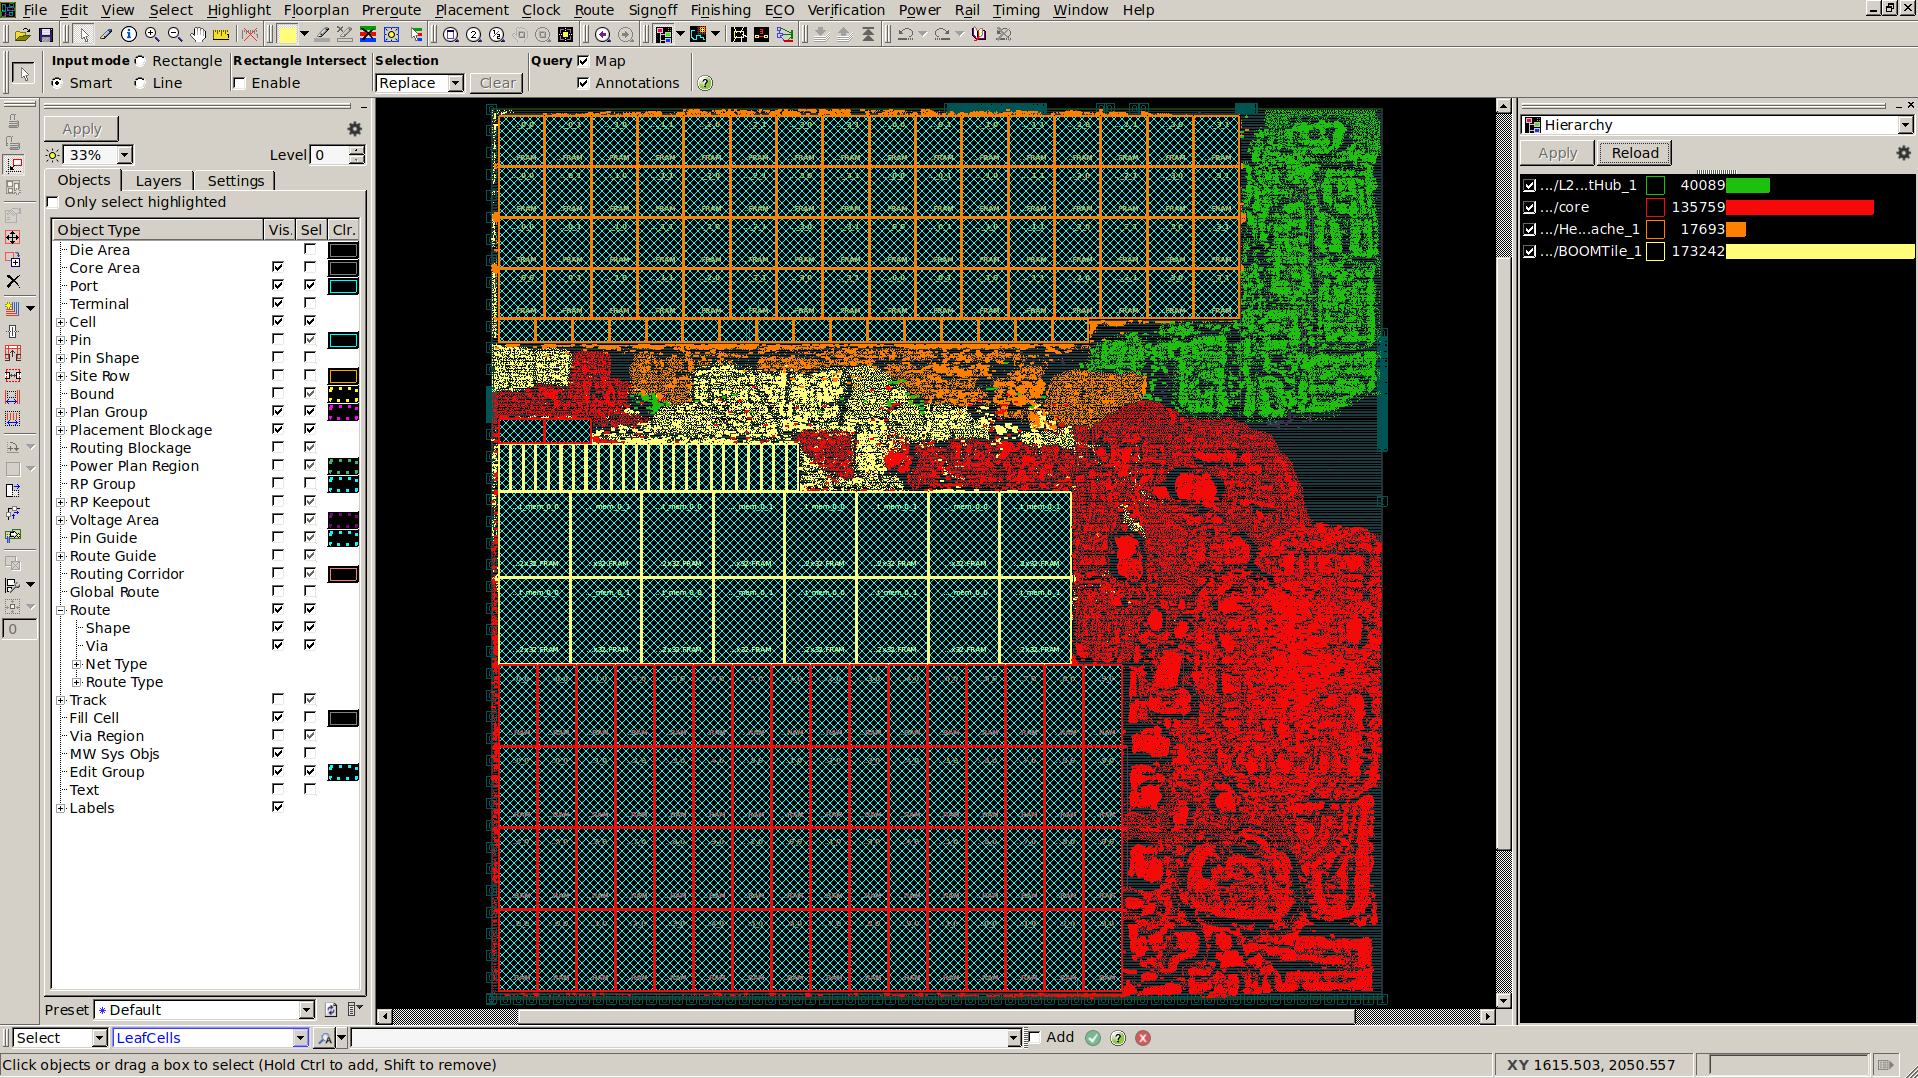
\includegraphics[width=0.95\linewidth]{figures/icc-boom.png}
  \end{center}
  \caption{ICC Floorplan for SmallBOOMConfig}
  \label{res:boom-icc}
\end{figure}

\begin{figure}
\begin{multicols}{2}
\begin{verbatim}
  Timing Path Group 'clock'
  -----------------------------------
  Levels of Logic:              53.00
  Critical Path Length:          3.56
  Critical Path Slack:          -1.56
  Critical Path Clk Period:      2.00
  Total Negative Slack:      -1282.67
  No. of Violating Paths:    10636.00
  Worst Hold Violation:          0.00
  Total Hold Violation:          0.00
  No. of Hold Violations:        0.00
  -----------------------------------
\end{verbatim}

\begin{verbatim}
  Cell Count
  -----------------------------------
  Hierarchical Cell Count:       1165
  Hierarchical Port Count:      76737
  Leaf Cell Count:             226528
  Buf/Inv Cell Count:           39474
  Buf Cell Count:               20757
  Inv Cell Count:               18717
  CT Buf/Inv Cell Count:         2089
  Combinational Cell Count:    187351
  Sequential Cell Count:        39177
  Macro Count:                    186
  -----------------------------------
\end{verbatim}

\begin{verbatim}
  Area
  -----------------------------------
  Combinational Area:   548249.859481
  Noncombinational Area:
                        260366.723512
  Buf/Inv Area:         141541.690599
  Total Buffer Area:         94002.53
  Total Inverter Area:       47539.16
  Macro/Black Box Area:
                       3912562.714844
  Net Area:            1230432.321193
  Net XLength        :     7458008.00
  Net YLength        :     7564863.50
  -----------------------------------
  Cell Area:           4721179.297837
  Design Area:         5951611.619030
  Net Length        :     15022872.00
\end{verbatim}
\end{multicols}
  \caption{ICC QoR Report for SmallBOOMConfig}
  \label{res:boom-qor}
\end{figure}

\subsection{Hwacha (with L2)}

\begin{figure}
  \begin{verbatim}
{
  "clocks": [
    {
      "name": "clock",
      "period": "2500ps",
      "par derating": "2500ps"
    }
  ],
  "scenerios": [
    {
      "corner": {
        "nmos": "typical",
        "pmos": "typical",
        "temperature": "25 C"
      },
      "supplies": {
        "VDD": "1.05 V",
        "GND": "0 V"
      }
    }
  ]
}
\end{verbatim}
  \caption{PLSI CAD Configuration for EOS24Config}
  \label{res:hwacha-config}
\end{figure}

\begin{figure}
\tiny
\begin{verbatim}
class HwachaTilePlacer(RocketTilePlacer):
  def __init__(self, config):
    self.top = None
    self.l1dd = []
    self.l1dm = []
    self.l1id = []
    self.l1im = []
    self.hid = []
    self.him = []
    self.hrf = []
    self.l2d = []
    self.l2m = []

  def insert(self, macro):
    if macro.matches(config.rtl_top):
      self.top = TopMacro(macro.name, macro.width, macro.height)
    elif macro.matches("DefaultCoreplex/tiles/HellaCache/data"):
      self.l1dd.append(macro)
    elif macro.matches("DefaultCoreplex/tiles/HellaCache/meta"):
      self.l1dm.append(macro)
    elif macro.matches("DefaultCoreplex/tiles/icache/icache"):
      self.l1id.append(macro)
    elif macro.matches("DefaultCoreplex/tiles/icache/icache/u"):
      self.l1id.append(macro)
    elif macro.matches("DefaultCoreplex/tiles/icache/icache/tag_array/tag_array"):
      self.l1im.append(macro)
    elif macro.matches("DefaultCoreplex/tiles/Hwacha/icache/icache"):
      self.hid.append(macro)
    elif macro.matches("DefaultCoreplex/tiles/Hwacha/icache/icache/u"):
      self.hid.append(macro)
    elif macro.matches("DefaultCoreplex/tiles/Hwacha/icache/icache/tag_array/tag_array"):
      self.him.append(macro)
    elif macro.matches("DefaultCoreplex/tiles/Hwacha/vus/vxuInst/laneInst/bankInst/rfInst/HwSRAMRF/HwSRAMR"):
      self.hrf.append(macro)
    elif macro.matches("DefaultCoreplex/tiles/Hwacha/vus/vxuInst/laneInst/bankInst/rfInst/HwSRAMRF/HwSRAMRF"):
      self.hrf.append(macro)
    elif macro.matches("DefaultCoreplex/L2HellaCacheBank/data_array/array"):
      self.l2d.append(macro)
    elif macro.matches("DefaultCoreplex/L2HellaCacheBank/meta/meta"):
      self.l2m.append(macro)
    else:
      print("%s cannot be matched" % macro.name)
      return False
    return True

  def list_constraints(self):
    l1dd = TopLeftPlacer   (self.top, self.top.tlf(), sorted(self.l1dd), True,  0.2)
    l1dm = TopLeftPlacer   (self.top, l1dd.bl(),      sorted(self.l1dm), False, 0.2)
    l1id = TopLeftPlacer   (self.top, l1dm.bl(),      sorted(self.l1id), False, 0.2)
    l1im = TopLeftPlacer   (self.top, l1id.bl(),      sorted(self.l1im), False, 0.2)
    hrf  = BottomLeftPlacer(self.top, self.top.blf(), sorted(self.hrf),  True,  0.2)
    hid  = BottomLeftPlacer(self.top, hrf.tl(),       sorted(self.hid),  False, 0.2)
    him  = BottomLeftPlacer(self.top, hid.tl(),       sorted(self.him),  False, 0.2)
    l2d  = TopRightPlacer  (self.top, self.top.trf(), sorted(self.l2d),  True,  0.8)
    l2m  = TopRightPlacer  (self.top, l2d.br(),       sorted(self.l2m),  False, 0.8)
    return l1dd.place() + l1dm.place() + l1id.place() + l1im.place() + hrf.place() + hid.place() + him.place() + l2d.place() + l2m.place()
\end{verbatim}
  \caption{PLSI Floorplan for EOS24Config}
  \label{res:rocket-fppy}
\end{figure}

\begin{figure}
  \begin{center}
    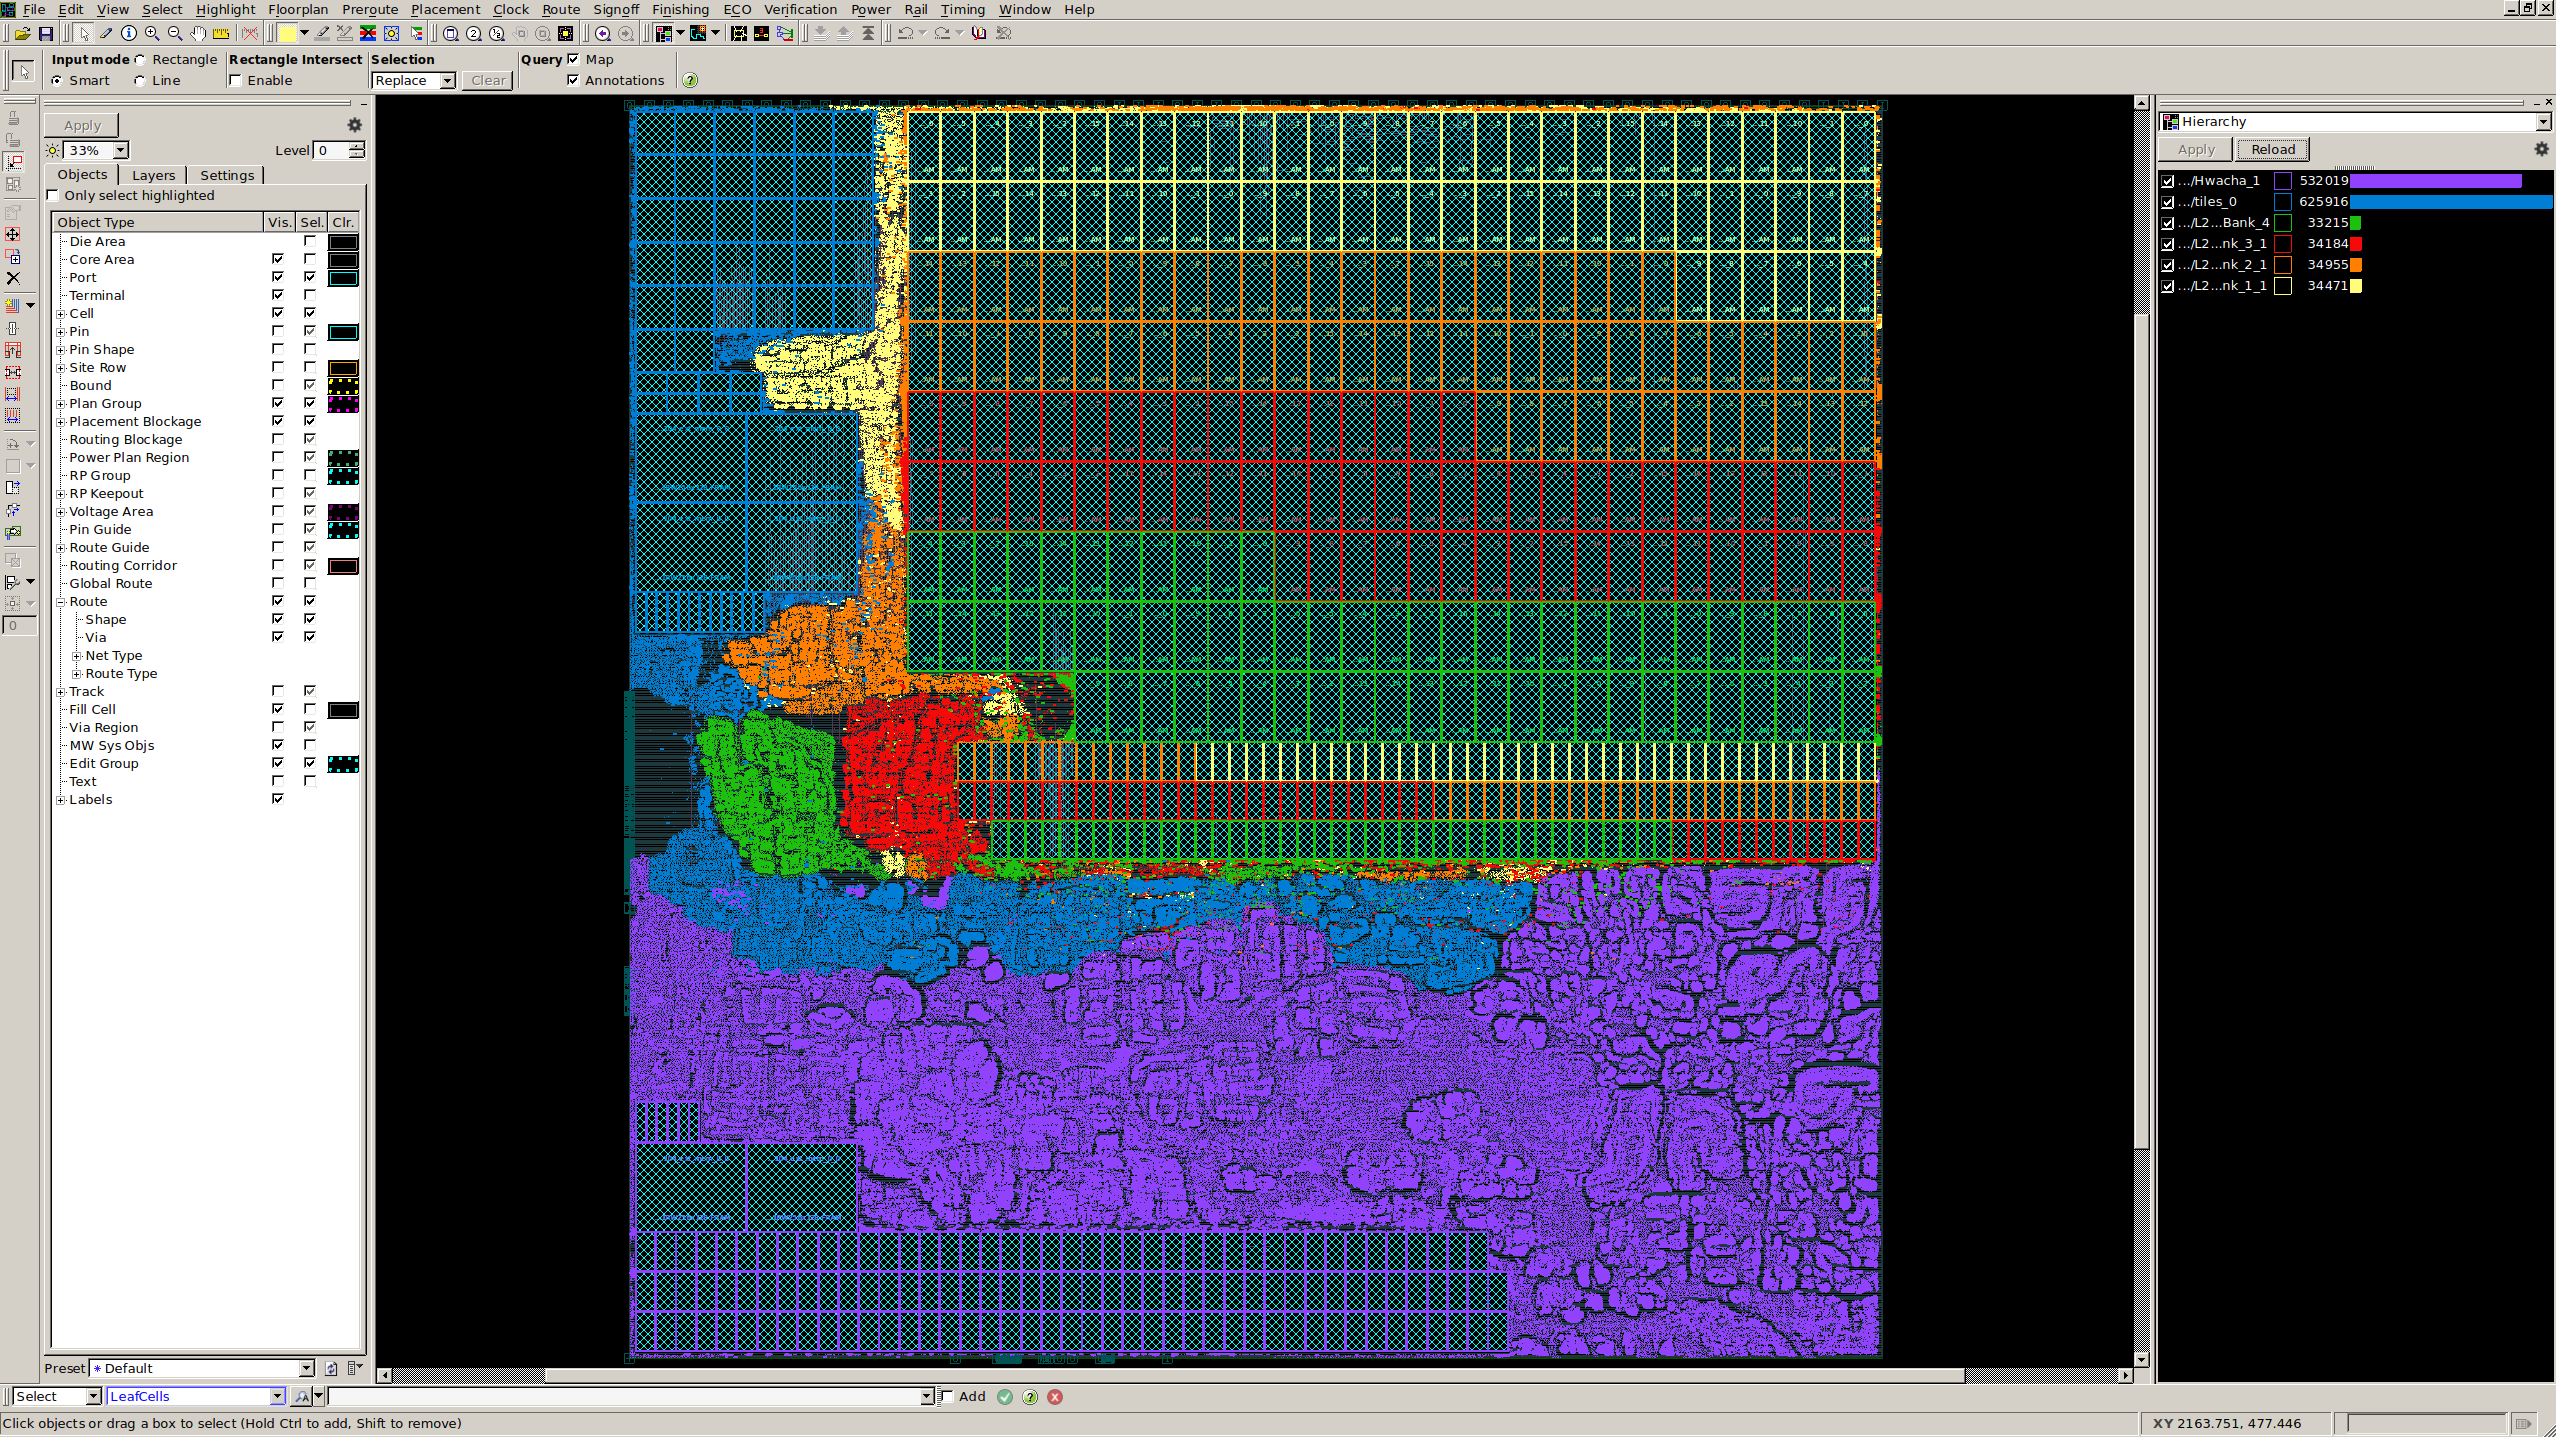
\includegraphics[width=0.95\linewidth]{figures/icc-hwacha.png}
  \end{center}
  \caption{ICC Floorplan for EOS24Config}
  \label{res:hwacha-icc}
\end{figure}

\begin{figure}
\begin{multicols}{2}
\begin{verbatim}
  Timing Path Group 'clock'
  -----------------------------------
  Levels of Logic:              29.00
  Critical Path Length:          5.63
  Critical Path Slack:          -0.73
  Critical Path Clk Period:      5.00
  Total Negative Slack:         -2.61
  No. of Violating Paths:       27.00
  Worst Hold Violation:          0.00
  Total Hold Violation:          0.00
  No. of Hold Violations:        0.00
  -----------------------------------
\end{verbatim}
\begin{verbatim}
  Cell Count
  -----------------------------------
  Hierarchical Cell Count:       3517
  Hierarchical Port Count:     145207
  Leaf Cell Count:             786039
  Buf/Inv Cell Count:          144033
  Buf Cell Count:               65811
  Inv Cell Count:               78222
  CT Buf/Inv Cell Count:         3501
  Combinational Cell Count:    686589
  Sequential Cell Count:        99450
  Macro Count:                    608
  -----------------------------------
\end{verbatim}
\begin{verbatim}
  Area
  -----------------------------------
  Combinational Area:  1875823.402210
  Noncombinational Area:
                        659483.367816
  Buf/Inv Area:         463893.370644
  Total Buffer Area:        283467.90
  Total Inverter Area:      180425.47
  Macro/Black Box Area:
                      10255909.371094
  Net Area:            3823554.904260
  Net XLength        :    28303776.00
  Net YLength        :    25156786.00
  -----------------------------------
  Cell Area:          12791216.141120
  Design Area:        16614771.045380
  Net Length        :     53460560.00


  Design Rules
  -----------------------------------
  Total Number of Nets:        850635
  Nets With Violations:         13080
  Max Trans Violations:          1133
  Max Cap Violations:           12164
\end{verbatim}
\end{multicols}
  \caption{ICC QoR Report for EOS24Config}
  \label{res:hwacha-qor}
\end{figure}

\section{Discussion}

The results in this section and meant to be suitable for doing computer
architecture research, not for building an actual chip.  As such they skip the
signoff sections of the flow that, from my experience when building chips,
don't have meaningful effects on QoR but take a lot of time to get right.

The simplest configuration run for this thesis was the default Rocket
configuration, DefaultConfig.  This contains Rocket, 64-bit a 5 stage in-order
core, with 32 KiB split L1 caches and a floating-point unit.  This
configuration and floorplan gets very good performance (1.5GHz) on commercial
28nm technologies, but it appears that the 32nm Synopsys EDK is significantly
slower.

The PLSI configuration used to generate DefaultConfig is shown in
Figure~\ref{res:rocket-config} and is pretty boring: there's a little bit of
derating for PAR, but that's just about as good as I'm able to do for anything.
The post-PAR results show that it's close to meeting timing, and that there
aren't too many DRC errors so the results are probably believable.

The Hwacha results are, however, a whole different story.  As you can see from
the PLSI configuration file, the physical design here gets very bad QoR --
there's a 50\% clock rate difference between the post-PAR and post-synthesis
results.  While some of this can be attributed to Rocket Chip's memories not
mapping well to the 32nm EDK's SRAMs (which have to write masks), a significant
part of this is probably due to the poor floorplan quality.  From looking at
Figure~\ref{res:hwacha-icc}, you can see how the floorplan generated from
Figure~\ref{res:hwacha-fppy} is quite bad: you can see how the L2 is too wide
and too short, which results in there being no space for the actual core logic.

\end{document}
